%
%
% Kapitel Datenstudie
%
%


\chapter{Vergleich der Monte-Carlo-Simulationen mit Daten}

\section{\texorpdfstring{$E_T$}{ET}-Spektren}

F�r elf der in Kapitel \ref{sec:montecarlo} erzeugten WHIZARD-Sample ($0\leq d_A^{\gamma} \leq 1$, Schritte von 0,1) werden nun die Hadronisierung und die Detektorantwort simuliert, die Rekonstruktionsalgorithmen darauf angewendet (siehe Abschnitt \ref{sec:reco}) sowie die in den Abschnitten \ref{sec:vorselektion} respektive \ref{sec:ttg_selektion} beschriebenen Selektionen durchgef�hrt. Die jeweiligen $E_T$-Spektren werden aufgetragen. Abb. \ref{fig:et_galerie} zeigt einige dieser Spektren in logarithmischer Auftragung, die $y$-Achse ist hier auf die Luminosit�t normiert. Man erkennt, dass wie erwartet das Spektrum mit steigendem $d_A^{\gamma}$ h�rter wird, sich also zu h�herenergetischen Photonen verschiebt. Dies l�sst sich auch in Abb. \ref{fig:et_kombi} erkennen, in der drei dieser Energiespektren �bereinandergeplottet sind. Des weiteren erkennt man eine Zunahme der Anzahl der rekonstruierten und selektierten Photonen mit steigender Kopplungsst�rke. Dies kommt zum einen daher, dass die $t\overline{t}+\gamma$-Selektion niederenergetische Photonen unterdr�ckt, zum anderen kann man hier auch auf eine Abh�ngigkeit des Wirkungsquerschnittes des Prozesses von $d_A^{\gamma}$ schlie�en, siehe \ref{sec:wq}. \\

\begin{figure}%
\begin{subfigure}[b]{0.4\textwidth}
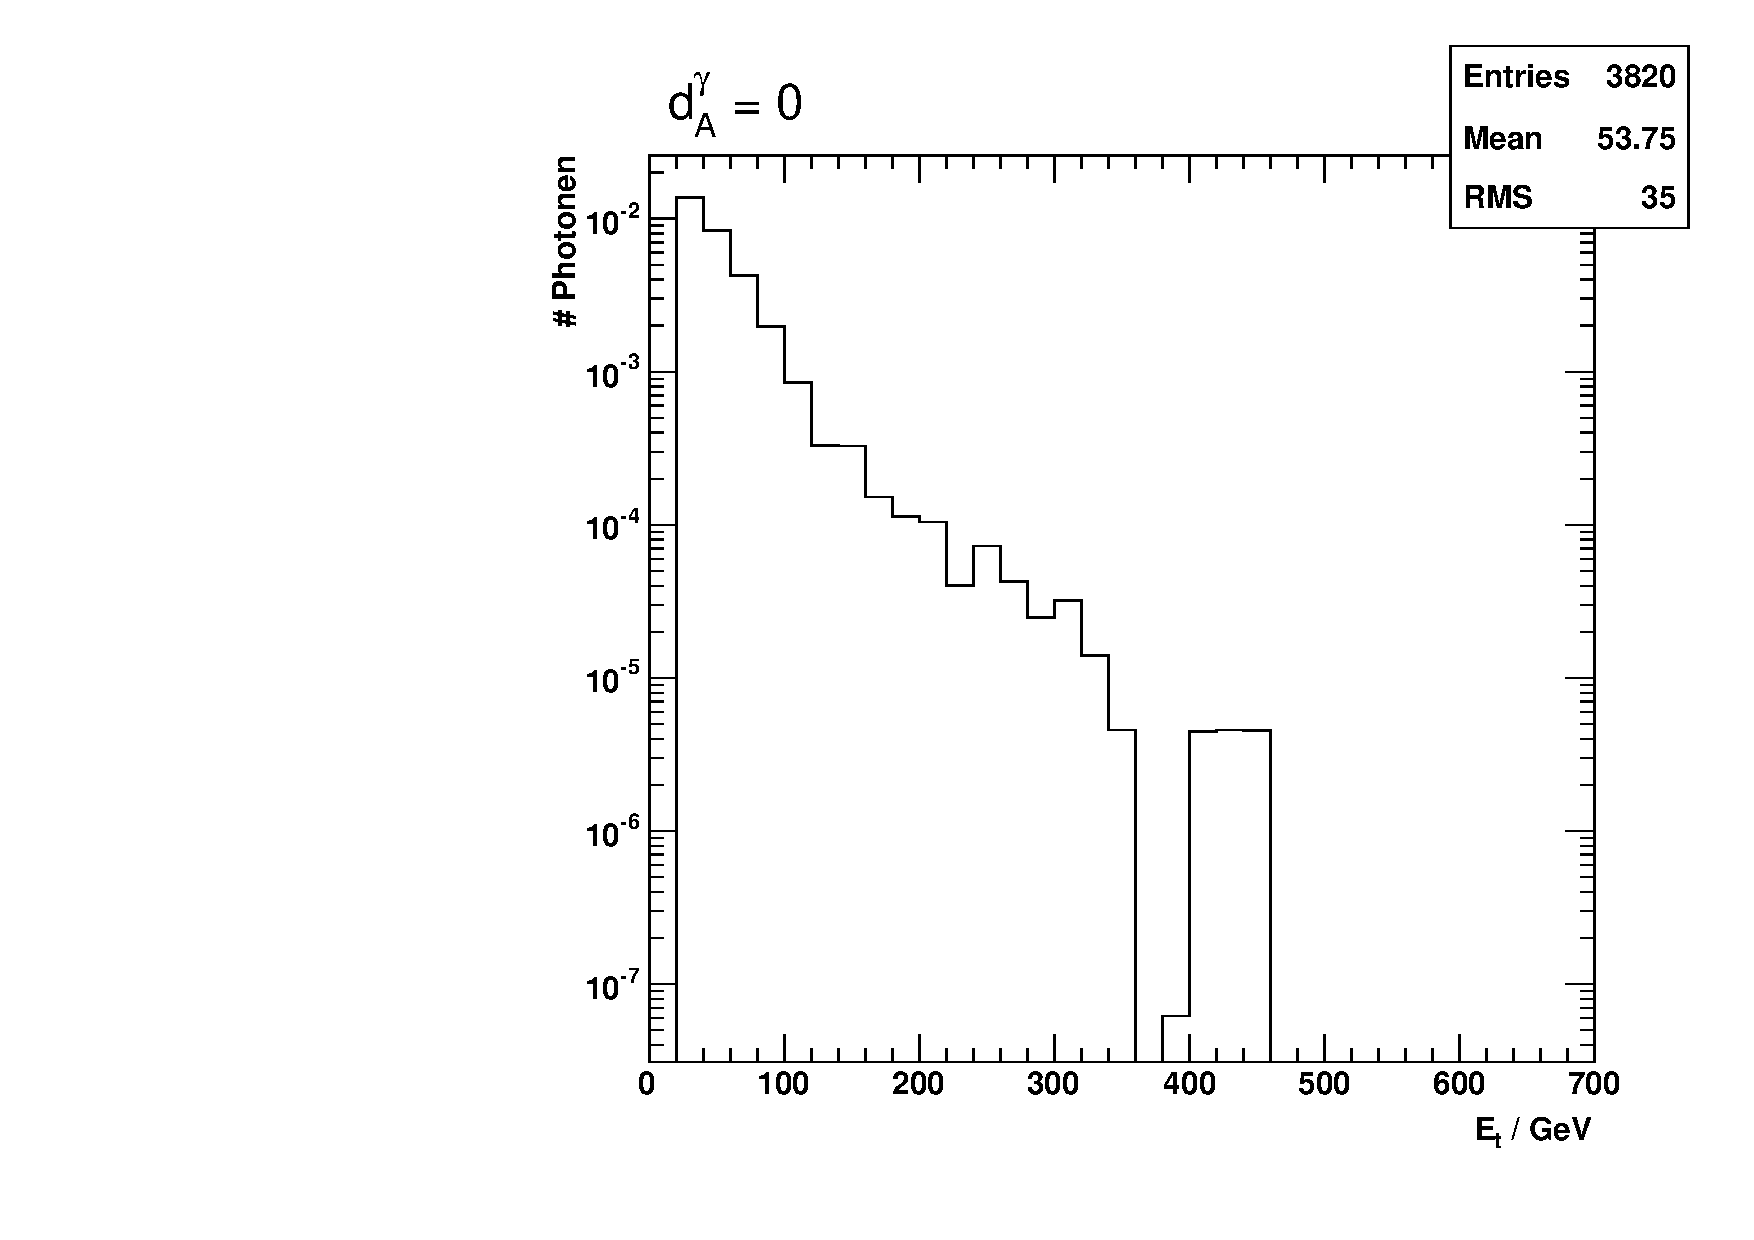
\includegraphics[width=\textwidth]{bilder/et_0}%
\end{subfigure}
\hspace{0.1\textwidth}
\begin{subfigure}[b]{0.4\textwidth}
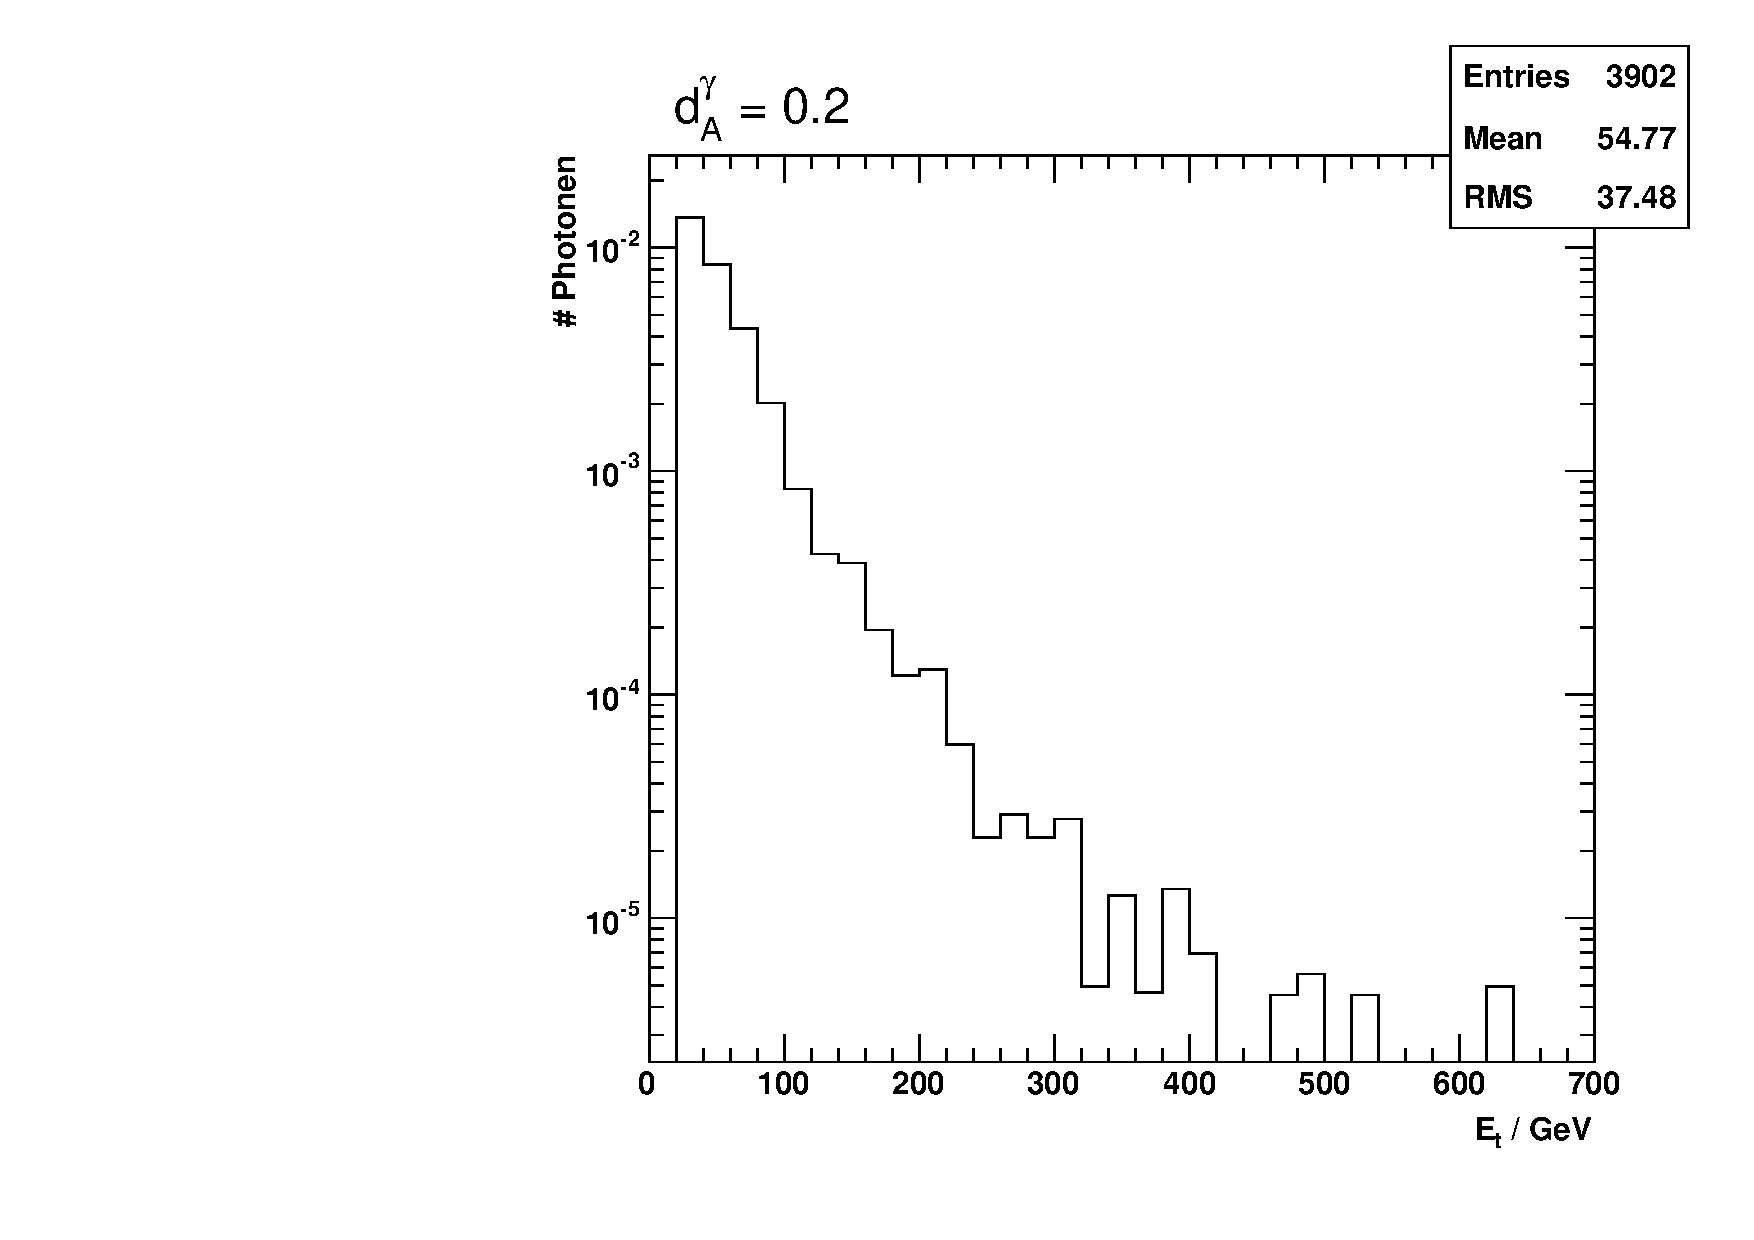
\includegraphics[width=\textwidth]{bilder/et_02}%
\end{subfigure}

\begin{subfigure}[b]{0.4\textwidth}
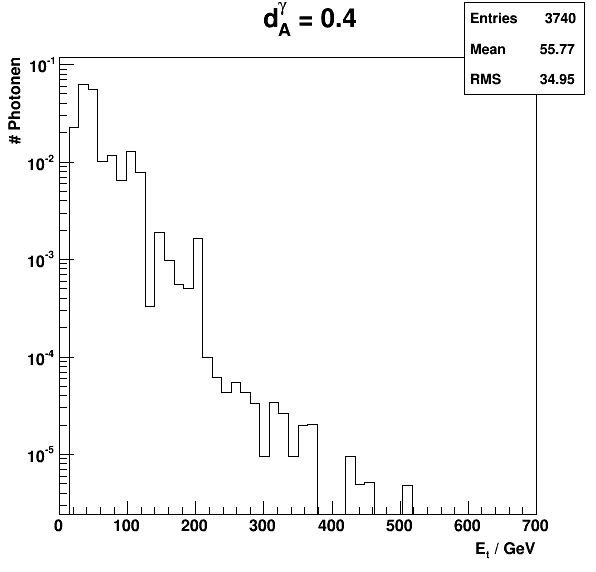
\includegraphics[width=\textwidth]{bilder/et_04}%
\end{subfigure}
\hspace{0.1\textwidth}
\begin{subfigure}[b]{0.4\textwidth}
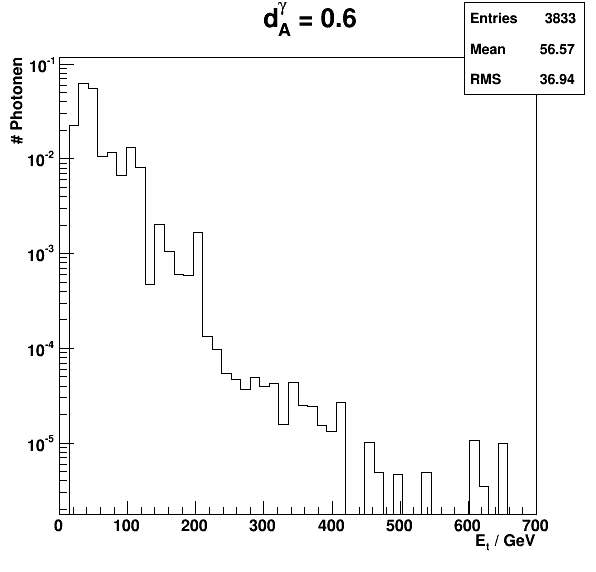
\includegraphics[width=\textwidth]{bilder/et_06}%
\end{subfigure}

\begin{subfigure}[b]{0.4\textwidth}
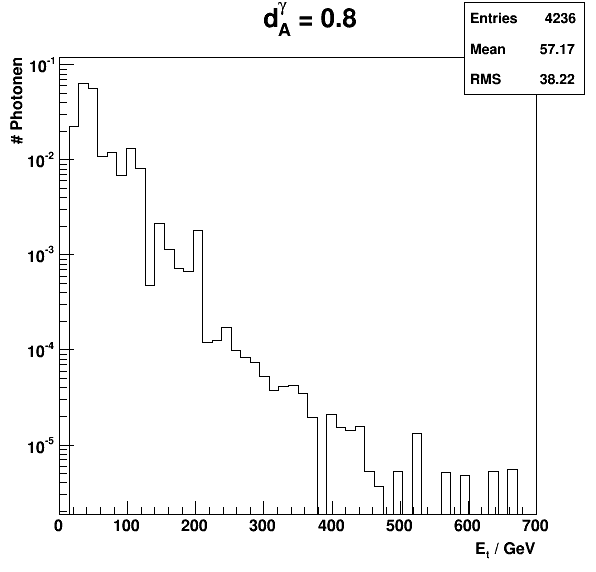
\includegraphics[width=\textwidth]{bilder/et_08}%
\end{subfigure}
\hspace{0.1\textwidth}
\begin{subfigure}[b]{0.4\textwidth}
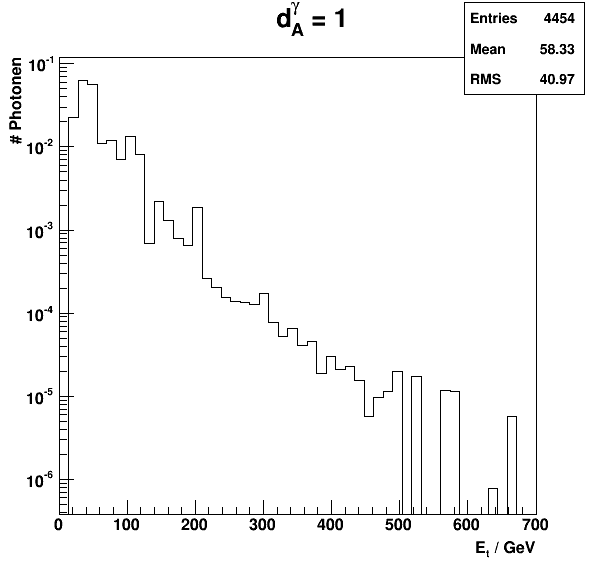
\includegraphics[width=\textwidth]{bilder/et_1}%
\end{subfigure}
\caption{$E_T$-Verteilungen von rekonstruierten und selektierten Monte-Carlo-Daten f�r verschiedene Werte von $d_A^{\gamma}$.}%
\label{fig:et_galerie}%
\end{figure}

\begin{figure}%
\centering

\includegraphics[width=0.4\columnwidth]{bilder/platzhalter}%
\caption{$E_T$-Spektren bei $d_A^{\gamma}=$0; 0,5 und 1.}%
\label{fig:et_kombi}%
\end{figure}

\section{Exponentieller Fit an die \texorpdfstring{$E_T$}{ET}-Spektren}

Von den in Kapitel \ref{sec:montecarlo} vorgestellten Analysemethoden, um den Wert von $d_A^{\gamma}$ anhand von Daten einzugrenzen, wird hier exemplarisch die Analyse der Einh�llenden der $E_T$-Verteilung der Photonen besprochen. Dazu wird nun an die prozessierten Monte-Carlo-Simulationen eine Exponentialfunktion

\begin{equation}
N(x) = N_0\cdot e^{\lambda \cdot x}
\end{equation}

 angefittet, siehe Abb. \ref{fig:fit_galerie}. Der Fitbereich liegt zwischen dem Bin mit der maximalen Anzahl der Eintr�ge bis 250\,GeV. Der Parameter$\lambda$ wird gegen $d_A^{\gamma}$ aufgetragen, siehe \ref{fig:et_slope}. Wie schon in Kapitel \ref{sec:ana_slope} wird nun ein Polynom dritten Grades an diese Datenpunkte gefittet, siehe Abb. \ref{fig:et_slopefit}. Man sieht, dass die Parameter ersten bis dritten Grades innerhalb der Unsicherheit des Fits mit Null vereinbar sind. Um dieser Problematik entgegenzuwirken, wird ein zweiter Ansatz mit einem linearen Fit gew�hlt. Dieser zeigt auch eine gute �bereinstimmung mit den Messwerten (Abb. \ref{fig:et_slopefit_linear}).  \\
In Abbildung \ref{fig:fehlerbandplot} sieht man die aus dem linearen Fit ermittelte Funktion 

\begin{equation}
\lambda\left(d_A^{\gamma}\right) = p_1\cdot d_A^{\gamma} +p_0 = 0,01069 \cdot d_A^{\gamma} -0,03916
\label{eq:lambda}
\end{equation}

(mittlere Gerade). Die obere und untere Gerade beschreibt respektive die Funktion f�r

\begin{equation}
\lambda\left(d_A^{\gamma}\right)_{max} = (p_1+\Delta p_1)\cdot d_A^{\gamma} +(p_0+\Delta p_0) = 0,01178 \cdot d_A^{\gamma} - 0,03842
\end{equation}

bzw. 

\begin{equation}
\lambda\left(d_A^{\gamma}\right)_{min} = (p_1-\Delta p_1)\cdot d_A^{\gamma} +(p_0-\Delta p_0) =  0,00960 \cdot d_A^{\gamma} - 0,03990 \ ,
\end{equation}

das so gebildete Fehlerband umschlie�t somit eine Standardabweichung.

\begin{figure}%
\begin{subfigure}[b]{0.4\textwidth}
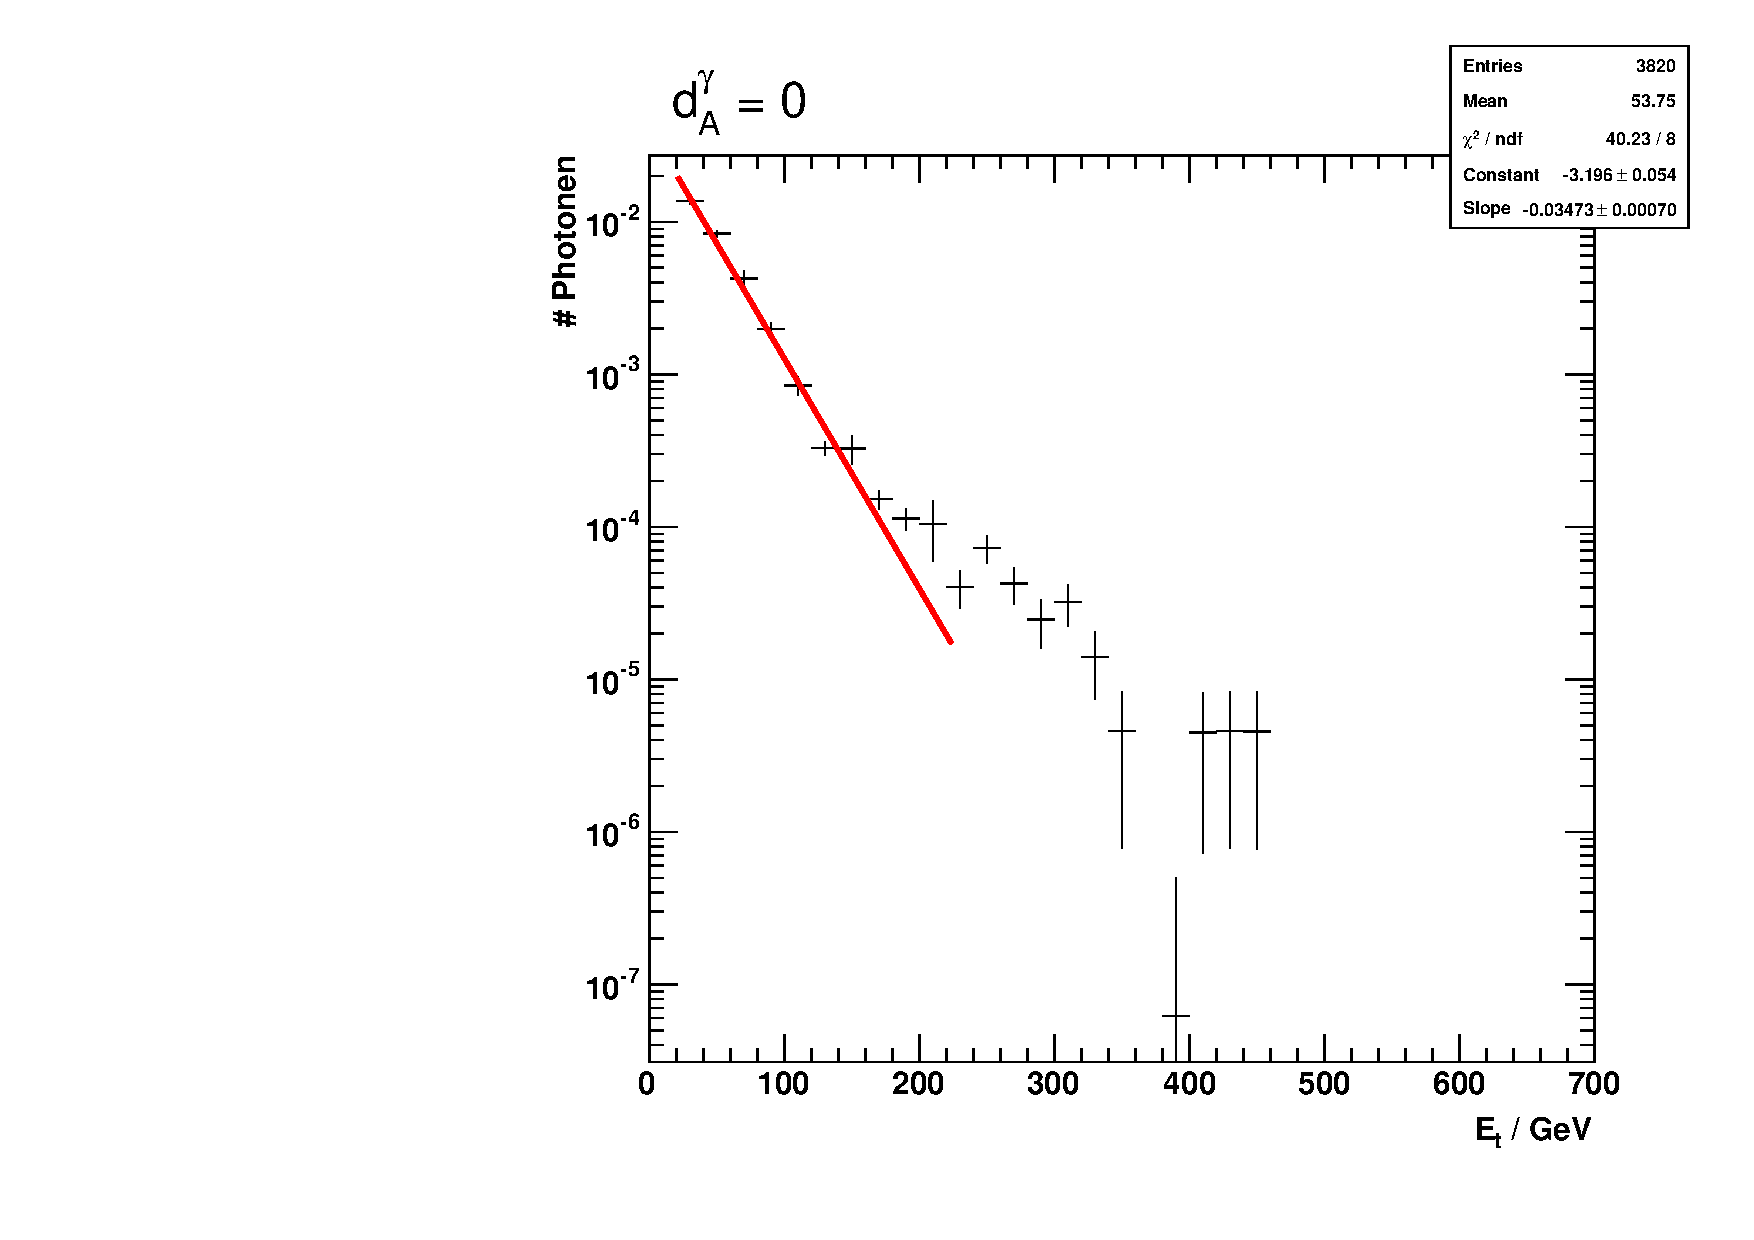
\includegraphics[width=\textwidth]{bilder/fit_0}%
\end{subfigure}
\hspace{0.1\textwidth}
\begin{subfigure}[b]{0.4\textwidth}
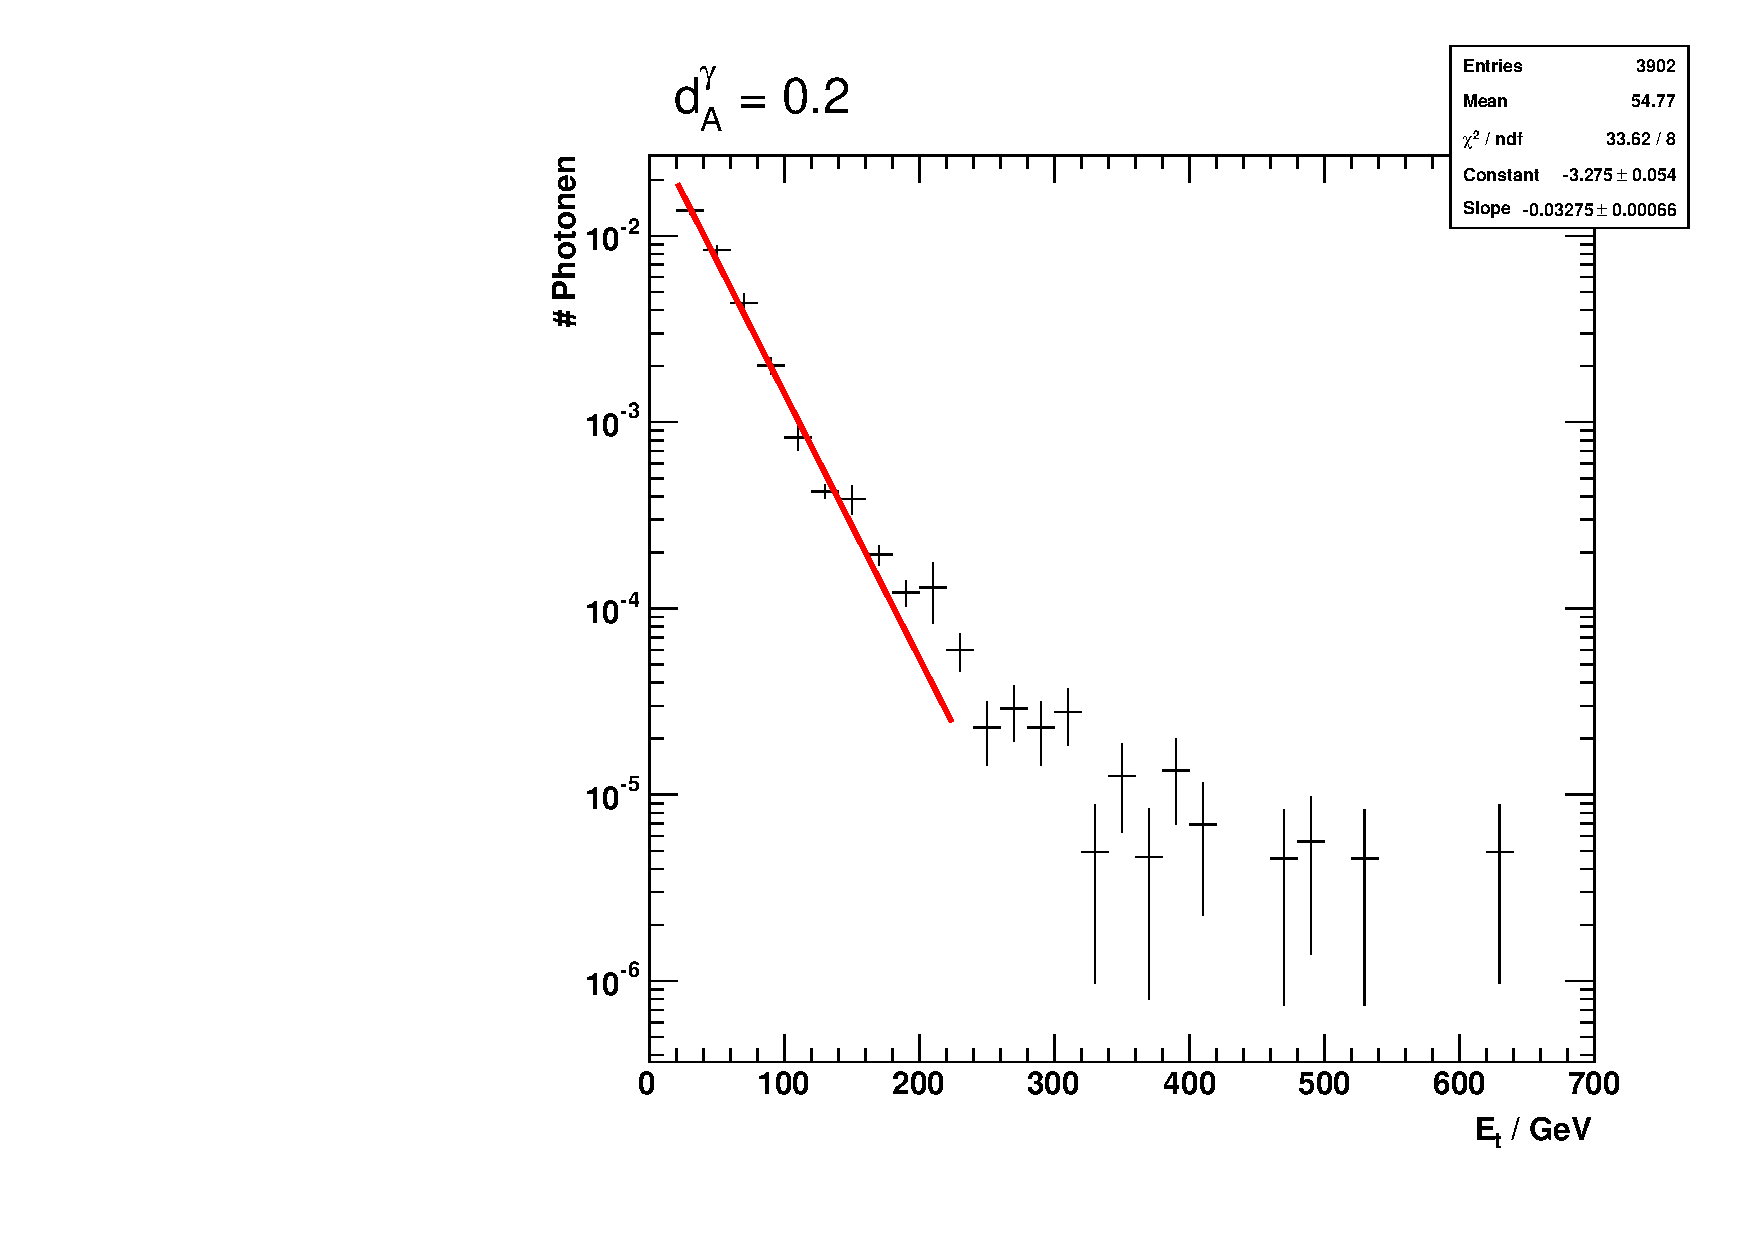
\includegraphics[width=\textwidth]{bilder/fit_02}%
\end{subfigure}

\begin{subfigure}[b]{0.4\textwidth}
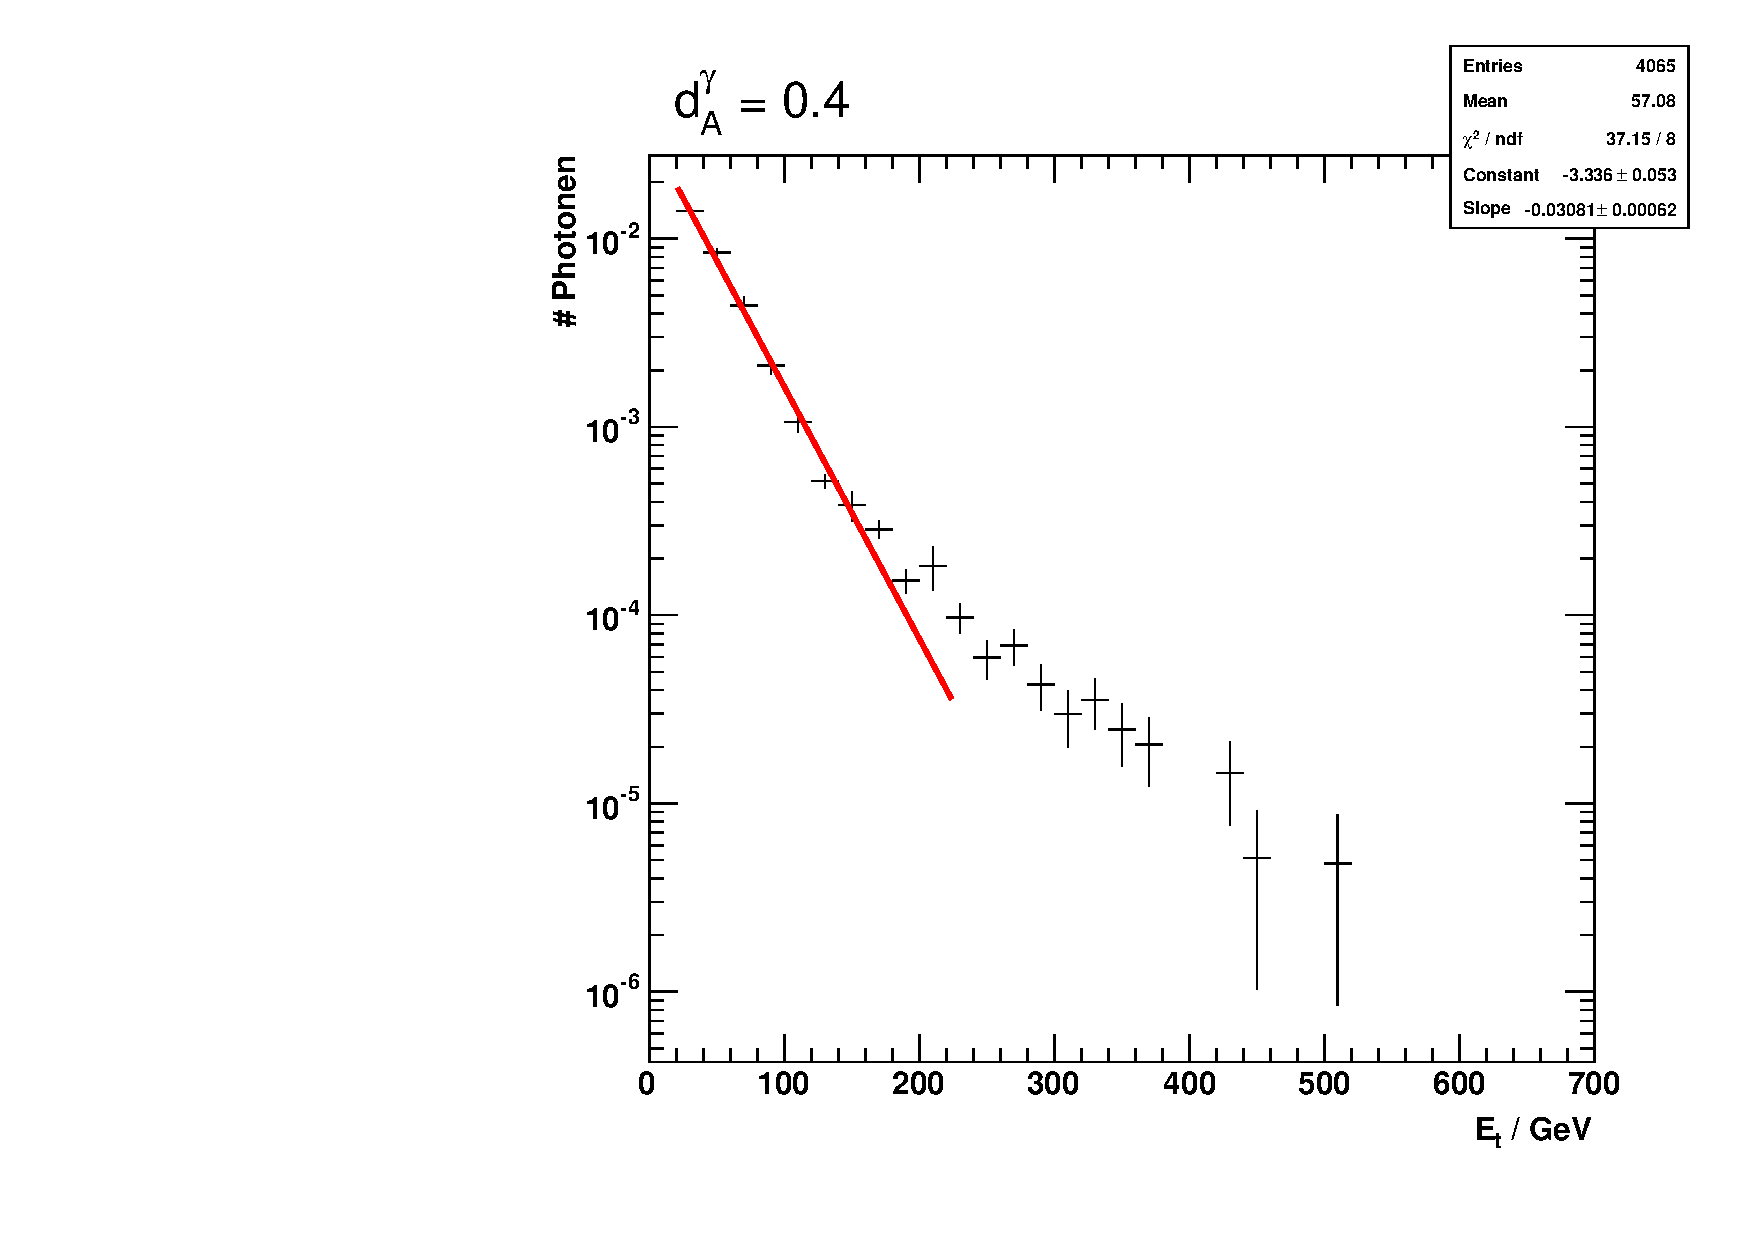
\includegraphics[width=\textwidth]{bilder/fit_04}%
\end{subfigure}
\hspace{0.1\textwidth}
\begin{subfigure}[b]{0.4\textwidth}
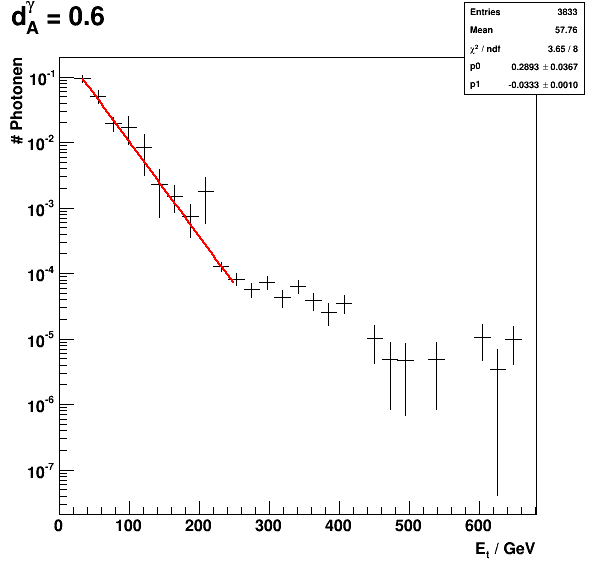
\includegraphics[width=\textwidth]{bilder/fit_06}%
\end{subfigure}

\begin{subfigure}[b]{0.4\textwidth}
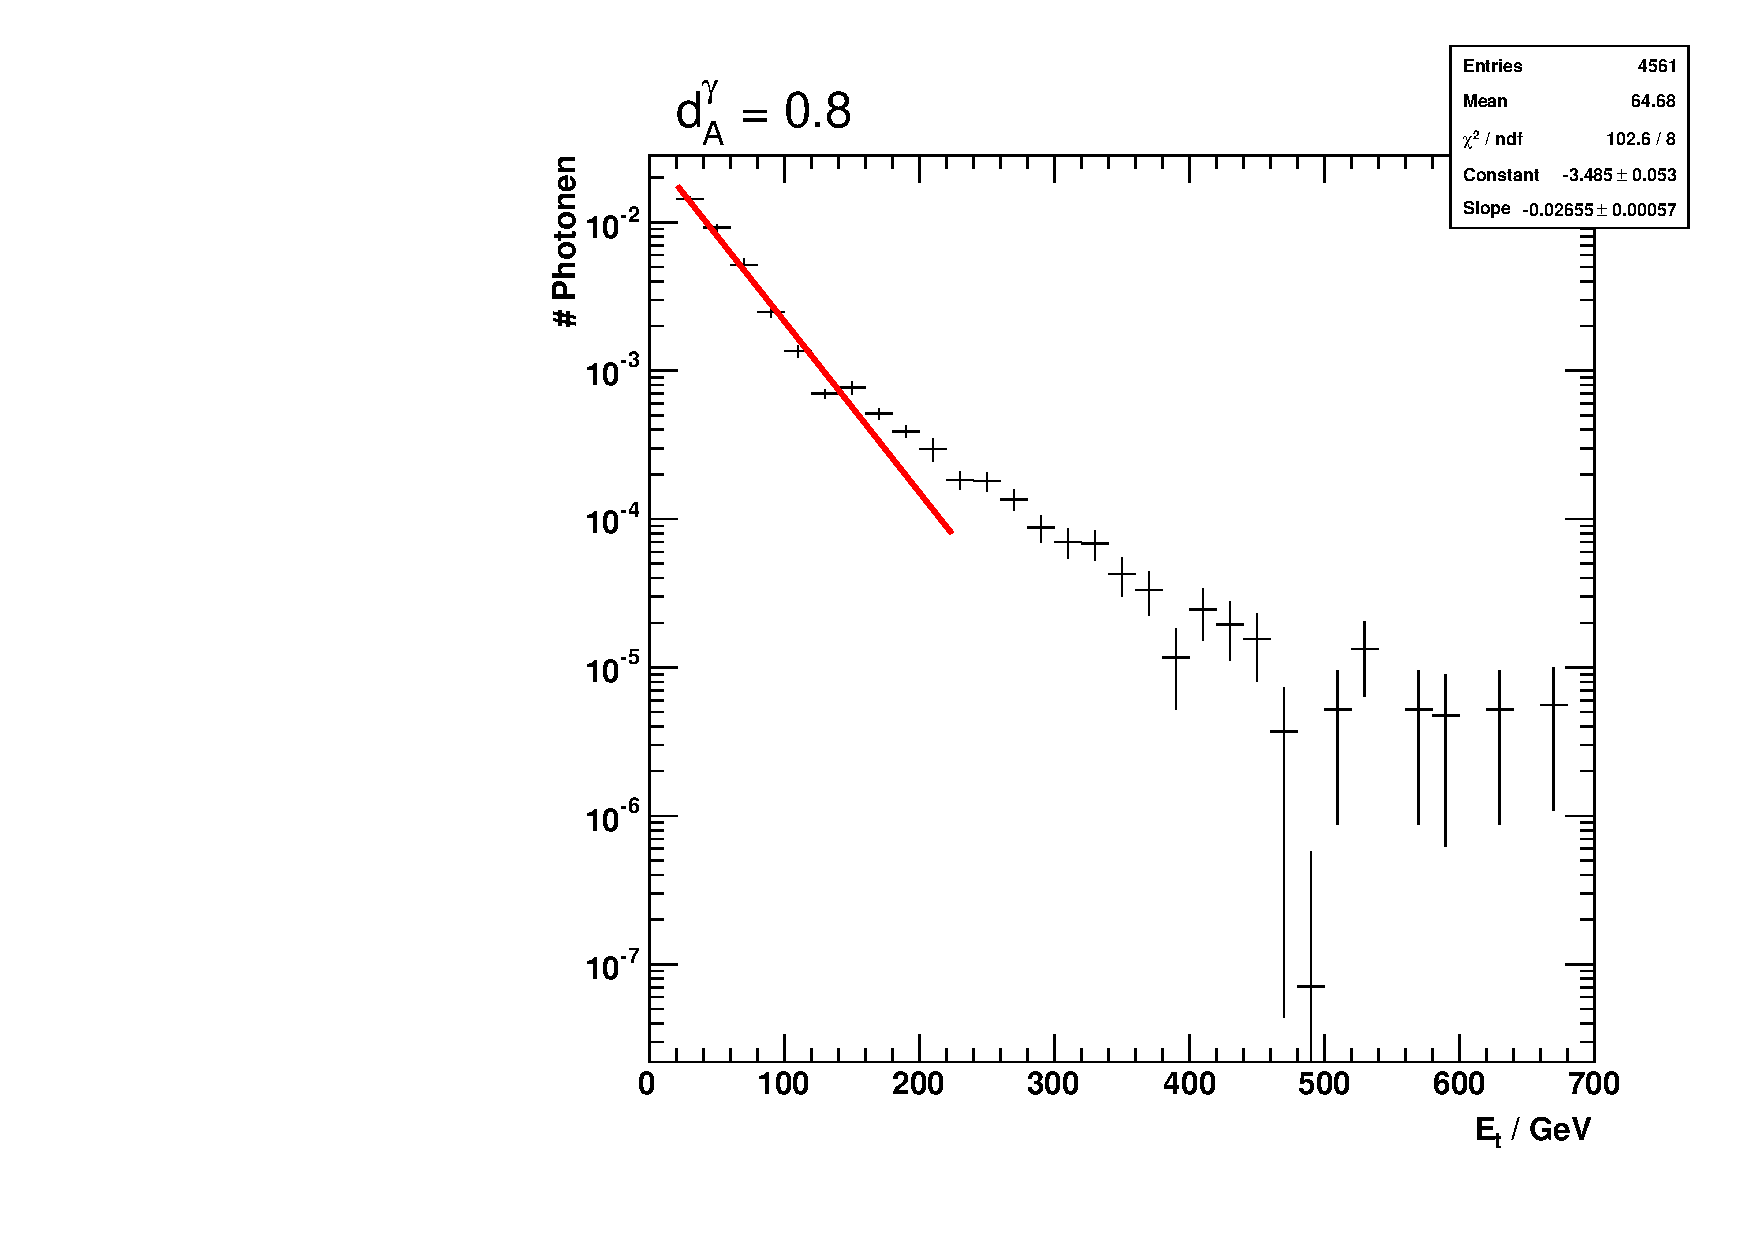
\includegraphics[width=\textwidth]{bilder/fit_08}%
\end{subfigure}
\hspace{0.1\textwidth}
\begin{subfigure}[b]{0.4\textwidth}
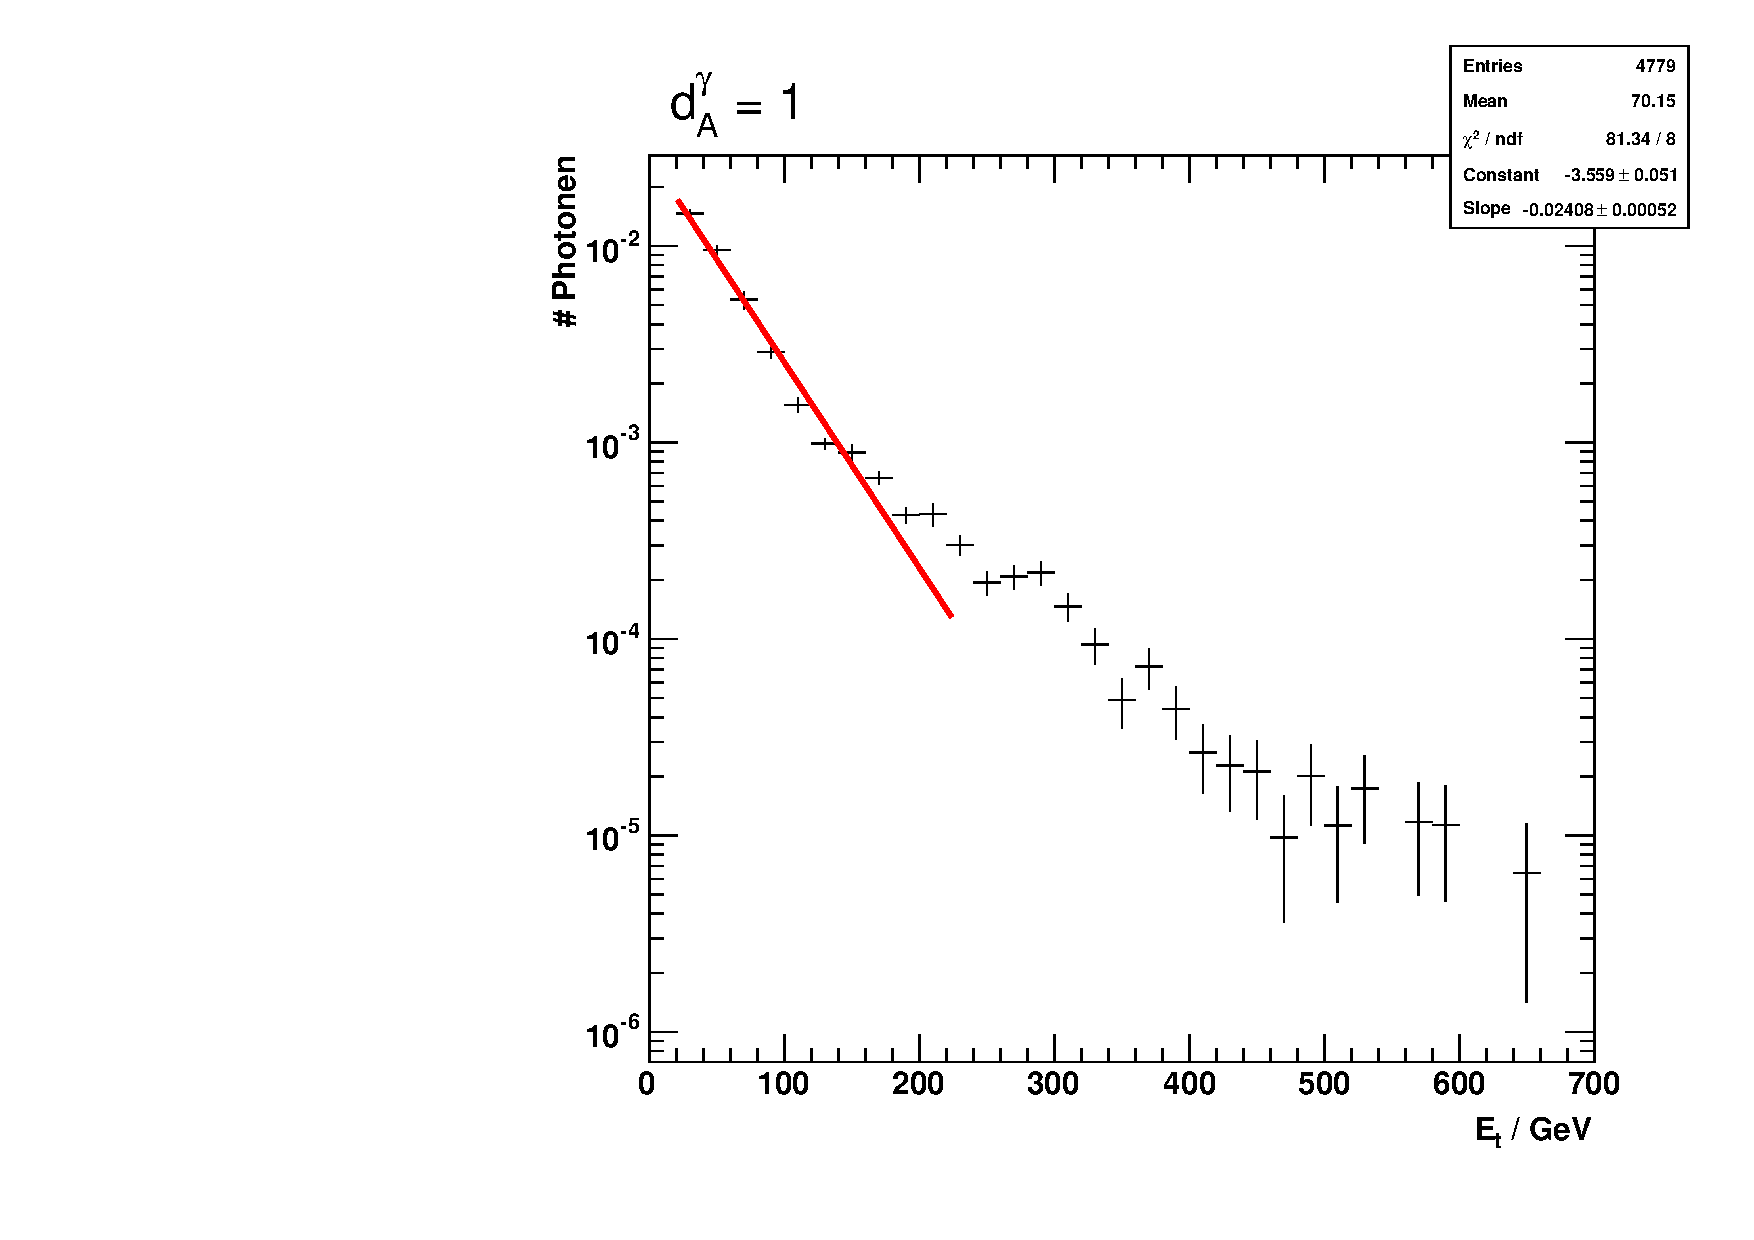
\includegraphics[width=\textwidth]{bilder/fit_1}%
\end{subfigure}
\caption{Exponentieller Fit an die $E_T$-Verteilungen von rekonstruierten und selektierten Monte-Carlo-Daten f�r verschiedene Werte von $d_A^{\gamma}$.}%
\label{fig:fit_galerie}%
\end{figure}

\begin{figure}%
\centering
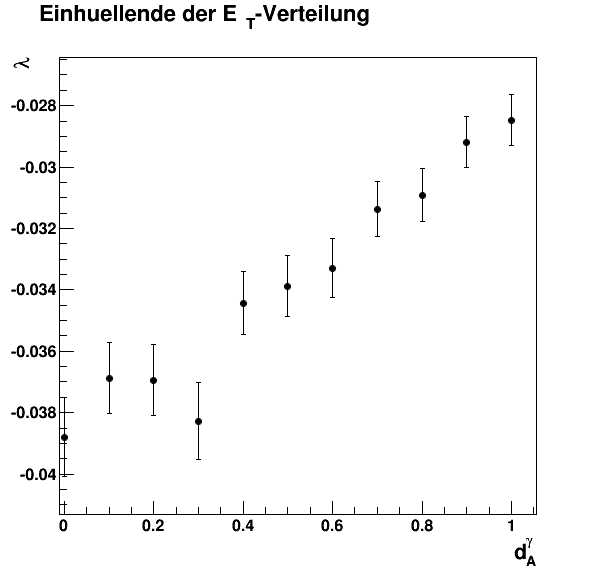
\includegraphics[width=0.4\columnwidth]{bilder/et_slope}%
\caption{Verlauf des $\lambda$-Parameters des Fits an die $E_T$-Spektren.}%
\label{fig:et_slope}%
\end{figure}

\begin{figure}%
\centering
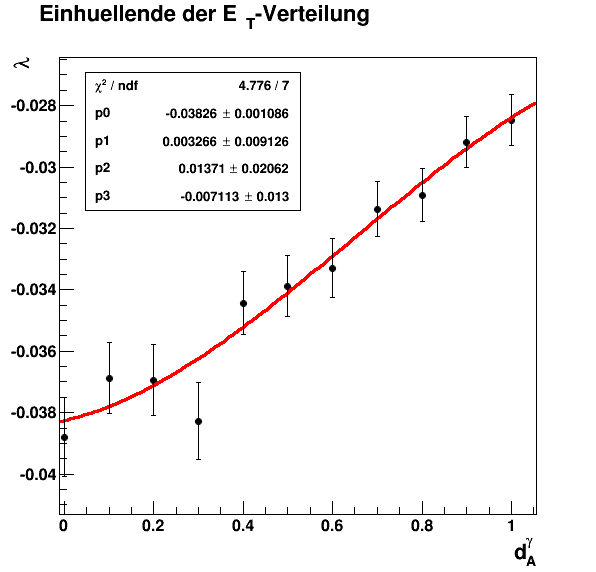
\includegraphics[width=0.4\columnwidth]{bilder/et_slopefit}%
\caption{Fit eines Polynoms dritten Grades an den Verlauf des $\lambda$-Parameters.}%
\label{fig:et_slopefit}%
\end{figure}

\begin{figure}%
\centering
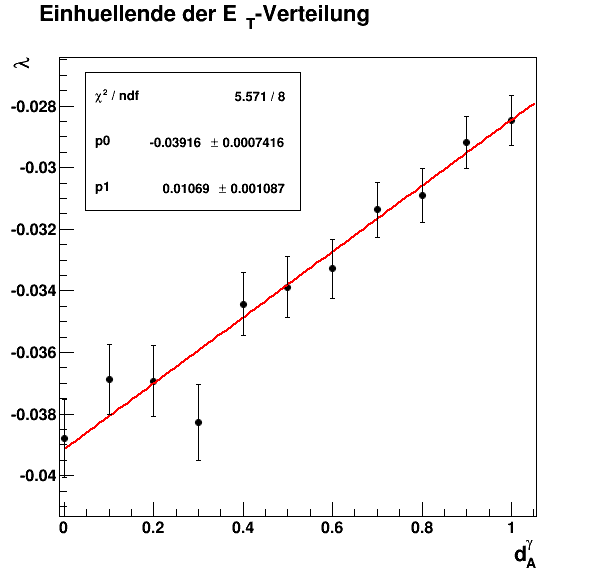
\includegraphics[width=0.4\columnwidth]{bilder/et_slopefit_linear}%
\caption{Linearer Fit an den Verlauf des $\lambda$-Parameters.}%
\label{fig:et_slopefit_linear}%
\end{figure}

\begin{figure}%
\centering
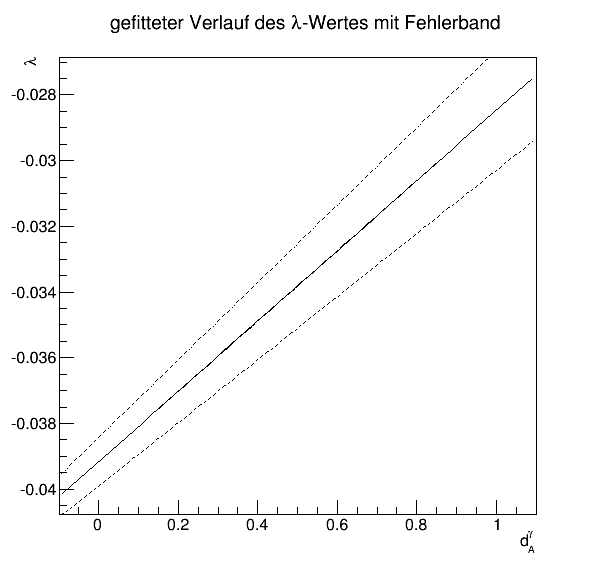
\includegraphics[width=0.4\columnwidth]{bilder/fehlerbandplot}%
\caption{Gefitteter Verlauf des $\lambda$-Wertes mit Fehlerband.}%
\label{fig:fehlerbandplot}%
\end{figure}

\section{Vergleich mit Daten}

Auf 4,7\,fb$^{-1}$ Daten werden die gleichen Selektionen (Top-Paar- bzw. $t\overline{t}+\gamma$-Selektion) angewendet. Die Daten wurden im Jahr 2011 bei einer Schwerpunktsenergie von 7\,TeV genommen. Aus diesem Datensatz werden 134 Ereignisse selektiert, die alle geforderten Kriterien erf�llen. Das $E_T$-Spektrum dieser Ereignisse ist in Abbildung \ref{fig:et_data} gezeigt. \\
Auch diese Verteilung wird nun mit einer Exponentialfunktion gefittet, diesen Fit zeigt Abbildung \ref{fig:et_data_fit}. Es ergibt sich f�r die Einh�llende ein Wert von

\begin{equation}
\lambda_{Data} = -0,03471 \cdot d_A^{\gamma} \pm 0,00366 \ .
\end{equation}

Die Genauigkeit dieses Fits ist durch die geringe Anzahl von nur 134 selektierten Ereignissen begrenzt. \\
Ziel ist es nun, durch Vergleich der Daten mit den Monte-Carlo-Simulationen einen Wert f�r $d_A^{\gamma}$ zu finden, der die gemessenen Daten repr�sentiert. Dazu wird aus der Umkehrfunktion von \ref{eq:lambda} $d_{A, Data}^{\gamma}$ bestimmt, siehe Abbildung \ref{fig:endplot}. Es ergibt sich ein Wert von 

\begin{equation}
d_{A, Data}^{\gamma} = 0,416_{-0,412}^{+0,506} \ .
\end{equation}



\begin{figure}%
\centering
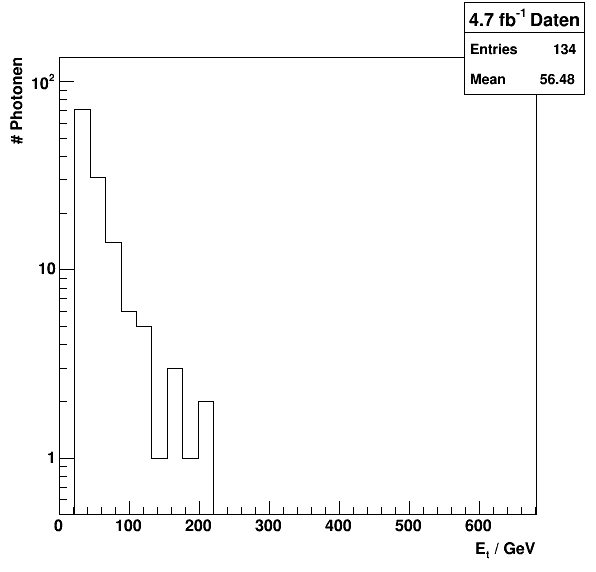
\includegraphics[width=0.4\columnwidth]{bilder/et_data}%
\caption{$E_T$-Verteilung von 4,7\,fb$^{-1}$ Daten aus 2011.}%
\label{fig:et_data}%
\end{figure}

\begin{figure}%
\centering
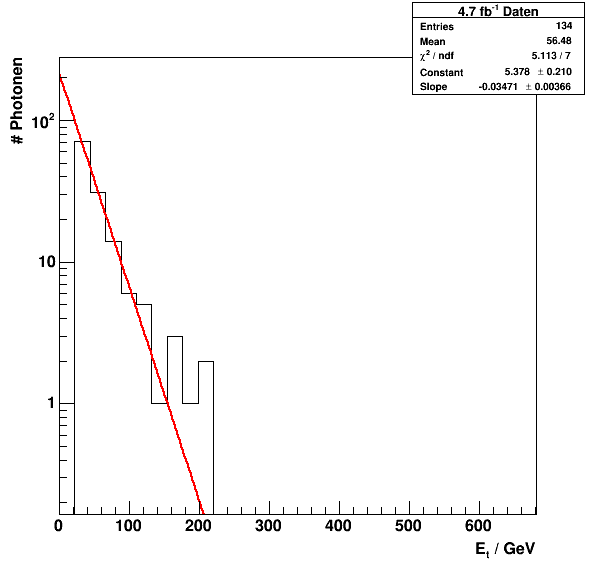
\includegraphics[width=0.4\columnwidth]{bilder/et_data_fit}%
\caption{Exponentialfit an die $E_T$-Verteilung von 4,7\,fb$^{-1}$ Daten aus 2011.}%
\label{fig:et_data_fit}%
\end{figure}

\begin{figure}%
\centering

\includegraphics[width=0.4\columnwidth]{bilder/platzhalter}%
\caption{Bestimmung des $d_{A, Data}^{\gamma}$-Parameters.}%
\label{fig:endplot}%
\end{figure}